\documentclass{article}
\usepackage{CJKutf8}

\usepackage{amsmath, amssymb}
% Set the page margins to 1 inch on all sides
\usepackage[a4paper, left=1in, right=1in, top=1in, bottom=1in]{geometry}
\usepackage{graphicx}
\usepackage{listings} 
\usepackage{dashrule}
\usepackage{color} %red, green, blue, yellow, cyan, magenta, black, white
\definecolor{mygreen}{RGB}{28,172,0} % color values Red, Green, Blue
\definecolor{mylilas}{RGB}{170,55,241}

\lstset{ 
	language=Matlab,                		% choose the language of the code
%	basicstyle=10pt,       			% the size of the fonts that are used for the code
%	numbers=left,                  			% where to put the line-numbers
	numberstyle=\footnotesize,      		% the size of the fonts that are used for the line-numbers
	stepnumber=1,                   		% the step between two line-numbers. If it's 1 each line will be numbered
	numbersep=5pt,                  		% how far the line-numbers are from the code
           keywordstyle=\color{blue},                   % choose the keyword color. You must add \usepackage{color}
           commentstyle=\color{black},                % choose the comment color. You must add \usepackage{color}
           stringstyle=\color{red},                         % choose the string color. You must add \usepackage{color}
%	backgroundcolor=\color{white},  	% choose the background color. You must add \usepackage{color}
	showspaces=false,               		% show spaces adding particular underscores
	showstringspaces=false,         		% underline spaces within strings
	showtabs=false,                 		% show tabs within strings adding particular underscores
%	frame=single,	                		% adds a frame around the code
%	tabsize=2,                			% sets default tabsize to 2 spaces
%	captionpos=b,                   			% sets the caption-position to bottom
	breaklines=true,                		% sets automatic line breaking
	breakatwhitespace=false,        		% sets if automatic breaks should only happen at whitespace
	escapeinside={\%*}{*)}          		% if you want to add a comment within your code
}

%Main 
\title{\vspace{-2cm}\Large Lecture Note 1: Plot Impulse Response Function with VAR model}
\author{Tai W}
\date{January 27, 2024}
\begin{document}
\begin{CJK}{UTF8}{gbsn}

\maketitle
\section*{Introduction}

An impulse-response function describes the evolution of the variables of interest along a specified time horizon after a shock in a given moment.

脉冲响应函数(Impulse Response Function)用于分析经济模型对外部冲击的动态响应,帮助我们理解当发生外部冲击的时候,模型的内生变量会随时间如何变化。这里将以三个变量的模型为例,GDP,居民消费,政府支出。我们将研究,政府支出对国家GDP与居民消费的影响,并在Matlab中绘制IRF图形。

\begin{figure}[!h]
    \centering
    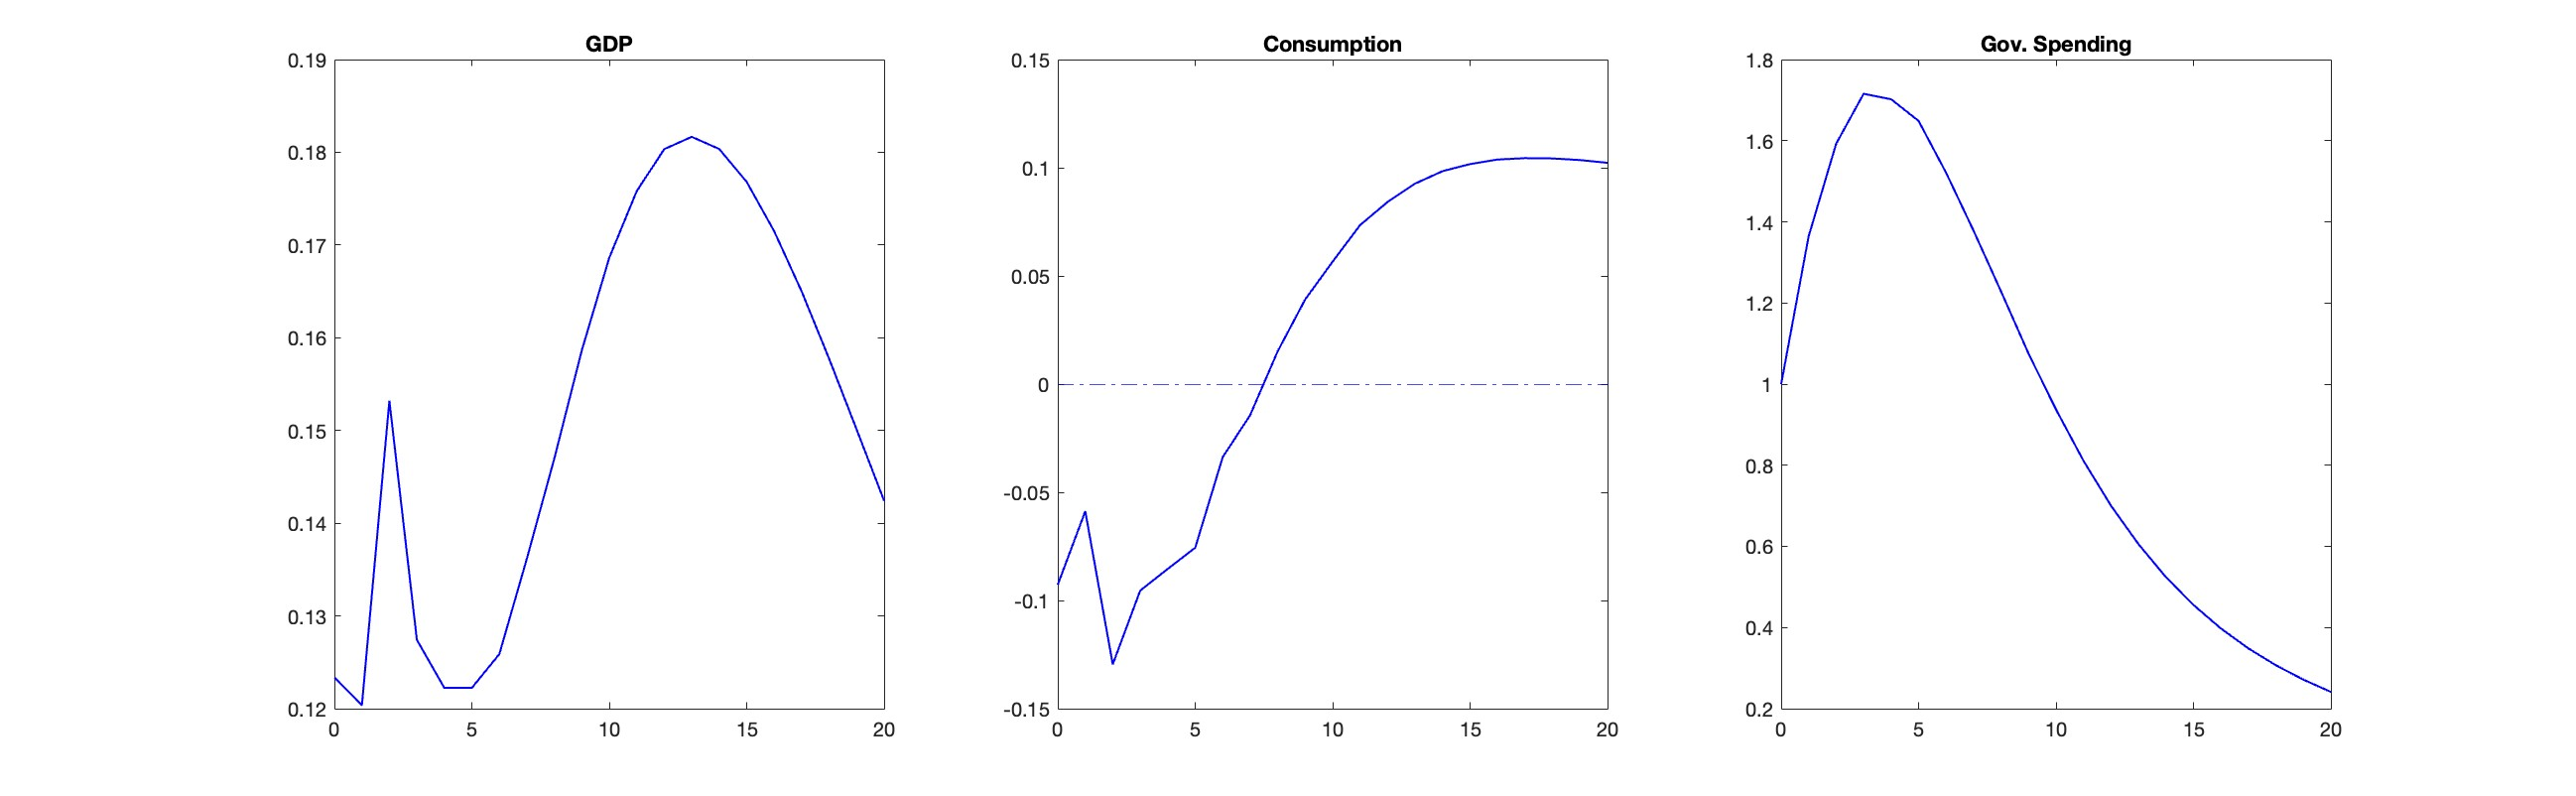
\includegraphics[width=1\linewidth]{Qb_1.jpg}
    \caption{Impulse Response Function for Government Spending Shock}
    \label{fig:enter-label}
\end{figure}

\section*{理论部分}
\section*{Univariate AR(1) Process}

Consider a univariate AR(1) process defined as:
\begin{equation}
    x_t = \phi x_{t-1} + u_t
\end{equation}
where $x_t$ is a scalar, $\phi < 1$ (which ensures the process is stationary) and $u_t$ is a (scalar) random disturbance with mean 0.

AR(1),是一阶自回归模型,即当前值与前一期的值存在线性关系。\( X_t\) 为当前值, \( X_{t-1}\) 为前一期的值。 \( \alpha \) 和\(\beta\) 是参数。 这里\(u_t\) 为模型的误差项(residual)。 

\subsection*{Stationary Process Representation}

For the stationary process, we can represent the AR(1) process as an infinite Moving Average (MA) representation. The lag operator $L$ is defined such that:
\begin{align*}
    Lx_t &= x_{t-1}, \\
    L^2x_t &= x_{t-2}.
\end{align*}
Thus, the AR(1) process can be written as:
\begin{equation}
    x_t = \frac{1}{1-\phi L}u_t
\end{equation}
By utilizing the geometric sum, we have:
\begin{equation}
    \frac{1}{1 - \phi L} = \sum_{i=0}^{\infty} (\phi L)^i
\end{equation}
对于平稳的时间序列,AR模型可以写成MA的形式,推理过程用到了等比数列求和公式。 
\begin{equation}
    x_t = u_t + \phi u_{t-1} + \phi^2 u_{t-2} + \phi^3 u_{t-3} + \cdots
\end{equation}

\section*{Vector Autoregression (VAR(1))}

If $x_t$ is not a scalar but a column vector with dimension $n \times 1$, then we have a VAR(1) model, which means a vector of interest variable with lag 1.
这里我们的模型中共有三个时间序列,GDP(\(y_t\)), Private Consumption(\(c_t\)), Government Spending(\(g_t\))。

\subsection*{Structure VAR}

For VAR, the structure equation is:
\begin{equation}
    A_0x_t = \alpha + \beta t + \sum_{i=1}^{p} A_ix_{t-i} + \varepsilon_t
\end{equation}
Here, $\varepsilon_t$ represents the structural shock.

\subsection*{Reduced Form VAR}

For the reduced form of VAR, the equation is:
\begin{equation}
    x_t = \alpha + \beta t + \sum_{i=1}^{p} B_ix_{t-i} + u_t
\end{equation}

 $u_t$ represents the reduced-form innovations, and structural shock is denoted by $\varepsilon_t$. We can relate them by:
 
\begin{equation}
    u_t = A_0^{-1} \varepsilon_t
\end{equation}
where  $\alpha$ is a constant regress, $\beta$ measures the time effect.

\section*{Impulse-Response Function}

The response of variables in $x$ in period $t$ to a shock in time $t$ (contemporaneous impact) is given by:

\begin{equation}
    x_t = B\varepsilon_t + \phi B\varepsilon_{t-1} + \phi^2 B\varepsilon_{t-2} + \phi^3 B\varepsilon_{t-3} + \cdots
\end{equation}
\begin{equation}
    \frac{\partial x_t}{\partial \varepsilon_t} = B
\end{equation}

The response of variables in $x$ in period $t+1$ to a shock in time $t$ is given by:
\begin{equation}
    \frac{\partial x_{t+1}}{\partial \varepsilon_t} = \phi B
\end{equation}

An impulse-response function will be a plot of $\frac{\partial x_{t+j}}{\partial \varepsilon_t}$ for all $j = 0, \ldots, h$ where $h$ is the time horizon of our plot.

对于一个周期为h的IRF函数,  IRF$(X_{t+j})$ 表现了变量在时间$t+j$ 对于发生于时间$t$ 冲击的反应,例如当年第一季度政府支出对明年第四季度GDP的影响。

\newpage
\section*{Example}
\subsection*{Plotting the Impulse Response Function}
以美国1947年至2023年国家GDP,居民消费,政府总支出为例,政府支出冲击对GDP与居民消费的影响。

Suppose we have data for US GDP $y_t$, Consumption $c_t$, Government Spending $g_t$, from 1947Q1 - 2023Q3 all measured in natural logarithms and measured per capita.

\subsection*{Structure VAR}
Given the structure VAR:
\begin{equation}
    A_0X_t = \alpha + \beta t + \sum_{i=1}^{P} A_iX_{t-i} + \varepsilon_t
\end{equation}

where $\alpha$ is a vector of constants, $t$ is the time trend, and $P$ is the lag length.

Assume $A_0$ is:
\begin{equation}
    A_0 = \begin{bmatrix}
    1 & 0 & -0.1234  \\
    0 & 1 &  0.0927\\
    0 & 0 & 1 
    \end{bmatrix}
\end{equation}

The designed matrix is for simplifying questions, not designed for reality, which states an assumption that government spending shock have no contemporaneous effect on GDP shock and consumption shock. We want to estimate the impulse response function to a government spending shock for GDP and Consumption. Take the forecast horizon as 20 as an example.

本例中,我们假定政府支出的冲击不受GDP与居民消费的影响,通过线性回归我们可以到的$A0$矩阵的数据。
同时,我们默认已经得到了Reduced Form VAR的参数值($B_i$)。(该过程可以通过对历史数据的GDP,居民消费,政府支出通过线性回归得出,基于政府支出的冲击不受GDP与居民消费的影响的假设)

Recall the reduced-form VAR:
\begin{equation}
    X_t = \alpha + \beta t + \sum_{i=1}^{4} B_i X_{t-i} + A_0^{-1} \varepsilon_t
\end{equation}
where $X_t$ is a $3 \times 1$ vector of endogenous variables, $\alpha$ and $\beta$ are $3 \times 1$ vectors of intercepts and trends respectively, $B_i$ are $3 \times 3$ matrices of autoregressive coefficients, and $\varepsilon_t$ is a $3 \times 1$ vector of shocks.

在以上方程中,假定我们已经得出了矩阵$B_i$ 与矩阵$A_0$. (通过OLS对每一个时间序列线性回归),简化形式参数矩阵的表示:

\begin{equation}
    \gamma_{\text{reduced}} = 
    \begin{bmatrix}
        \alpha^{gdp} & \alpha^{cons} & \alpha^{gov} \\
        \beta^{gdp} & \beta^{cons} & \beta^{gov} \\
        B^{gdp}_{lag1gdp} & B^{cons}_{lag1gdp} & B^{gov}_{lag1gdp} \\
        \vdots & \vdots & \vdots \\
        B^{gdp}_{lag4gov} & B^{cons}_{lag4gov} & B^{gov}_{lag4gov}
    \end{bmatrix}
\end{equation}
where $\gamma_{\text{reduced}}$ is a $14 \times 3$ matrix and is the coefficient of VAR parameter.

结合我们的目前所有的信息,我们可以用以上参数来重新描述VAR模型。\\

Then we can write Reduced form $X_t$ as a combination of coefficients with predictors:
\begin{align*}
    X_t &= \gamma_{\text{reduced}}[Constant Coeffi] + \gamma_{\text{reduced}}[Time Coeffi]*t  \\
    &\quad + \gamma_{\text{reduced}}[Lag1]* X_{t-1} + \gamma_{\text{reduced}}[Lag2]* X_{t-2} \\
    &\quad + \gamma_{\text{reduced}}[Lag3]]*X_{t-3} + \gamma_{\text{reduced}}[lag4]*X_{t-4}\\
    &\quad + A_0^{-1} \varepsilon_t
\end{align*}

为了找到政府支出的 IRF,我们设定在时间 0 时的政府支出冲击设为 1,其他所有为 0;对于时间 t 不为 0,所有冲击设为 0。另外,注意在 t 为 1 的时候,仅有 1 个滞后效应(t=0),t 为 2 时,有两个(t=0, t= 1),以此类推...

\begin{align*}
IR(X_h) &= [\gamma^{\text{reduced}}]_{lag1} \times IR(X_{h-1}) + [\gamma^{\text{reduced}}]_{lag2} \times IR(X_{h-2}) \\
&+ [\gamma^{\text{reduced}}]_{lag_3} \times IR(X_{h-3}) + [\gamma^{\text{reduced}}]_{lag_4} \times IR(X_{h-4}) \\
&+ A_0^{-1} \times \varepsilon_h
\end{align*}

\begin{equation}
    \varepsilon_0 = \begin{pmatrix} 0 \\ 0 \\ 1 \end{pmatrix}, \quad
    \varepsilon_h = \begin{pmatrix} 0 \\ 0 \\ 0 \end{pmatrix} \text{ for all } h > 0, \quad h = 0, 1, 2, \ldots, 20,
\end{equation}

\begin{equation}
    IR(X_{-1}) = IR(X_{-2}) = IR(X_{-3}) = IR(X_{-4}) = \begin{pmatrix} 0 \\ 0 \\ 0 \end{pmatrix}.
\end{equation}

\section*{Matlab Code}
\begin{enumerate}
    \item 初始化一个 $3 \times 21$ 的矩阵来存放 IRF 的值,即观测周期从 $t = 0$ 到 $t = 20$。
    \item 用递归的方式得到 IRF($X_h$) ,对于 $t = 0, 1, 2, \ldots, 20$。
    \item 注意在 $t = 0$ 时,没有滞后效应,IRF 为初始状态 ${A_0^{-1} \varepsilon_t}$。
\end{enumerate}

\begin{lstlisting}
% Importing data
mydata = xlsread('Exer1_2024','Data'); % Import data from Excel file to MATLAB 

% We need the per capita data so drop the pop is missing 
% Identify the rows where the population data (column 5) is NaN
rowsWithNaNInPop = isnan(mydata(:, 28));
% Remove those rows from the dataset
mydata(rowsWithNaNInPop, :) = [];

log_GDP = log(mydata(:,2));
log_Private_Sector_Consumption = log(mydata(:,3));
log_Government_Spending = log(mydata(:,23));

% Measuring all in per capita
GDP = log_GDP - log(Pop);
Consumption = log_Private_Sector_Consumption - log(Pop);
Government = log_Government_Spending - log(Pop);

    
% Initialize the matrix of regressors
X = [ones(length(TIME),1), TIME]; % Add a constant and time trend
 
% Generate lagged variables for each lag order
lags = 4; % 4 lags
for i = 1:lags
        X = [X, ...
             lagmatrix(GDP, i), ...
             lagmatrix(Consumption, i), ...
             lagmatrix(Government, i)];
end

\end{lstlisting}

\begin{lstlisting}
% Remove rows with NaN values that result from lagging
validRows = ~any(isnan(X), 2); % not ~, retrun True if not non, False if contains non
X = X(validRows, :);
    
GDP         = GDP(validRows);
Consumption = Consumption(validRows);
Government  = Government(validRows);

% Display result for Question 1
disp(repmat('-', 1, 60))
disp(["Answer for Question 1a "])
 
% Initial A0 
A0 = [1, 0, -0.1234; 
      0, 1, 0.0927;
      0, 0, 1]

%Find inverse 
inverseA = inv(A0); 

% The beta_matrix is take as given or Run OLS 
beta_matrix = [beta_GDP, beta_Consumption, beta_Government]; %Full sample parameter 
\end{lstlisting}

\begin{figure}[!h]
    \centering
    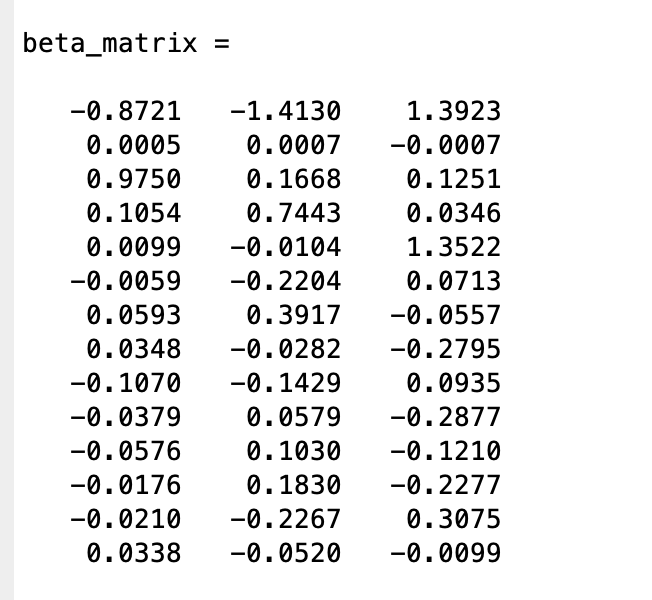
\includegraphics[width=0.5\linewidth]{Reduced VAR Coefficient Matrix .png}
    \caption{Reduced VAR Coefficient Matrix 14*3}
    \label{fig:enter-label}
\end{figure}

\begin{lstlisting}
%initial irf matrix 
h = 20; % windows = 20 
cal_IRF = zeros(3,h+1); %extend one for period 0

%get gamma_lag_1, gamma_lag_2, gamma_lag_3, gamma_lag_4
gamma_lag_1 = beta_matrix(3:5,1:3)';
gamma_lag_2 = beta_matrix(6:8,1:3)';
gamma_lag_3 = beta_matrix(9:11,1:3)';
gamma_lag_4 = beta_matrix(12:14,1:3)';

%Initial Shocks
epsilon_shock = zeros(3,h+1); % extend one for period 0
epsilon_shock(3,1) = 1;
% Loop For IRF 
for i = 1:h+1  
    if i == 1 %X0
        cal_IRF(:,i) = inverseA * epsilon_shock(:,i);  % Initial impact
    
    elseif i == 2 %X1
        cal_IRF(:,i) = gamma_lag_1 * cal_IRF(:,i-1);
    
    elseif i == 3 %X2
        cal_IRF(:,i) = gamma_lag_1 * cal_IRF(:,i-1) + gamma_lag_2 * cal_IRF(:,i-2);
    
    elseif i == 4% X3
        cal_IRF(:,i) = gamma_lag_1 * cal_IRF(:,i-1) + gamma_lag_2 * cal_IRF(:,i-2) + gamma_lag_3 * cal_IRF(:,i-3);
    else
        % For periods 5 and beyond, we use all four lags
        cal_IRF(:,i) =  gamma_lag_1 * cal_IRF(:,i-1) + ...
                        gamma_lag_2 * cal_IRF(:,i-2) + ...
                        gamma_lag_3 * cal_IRF(:,i-3) + ...
                        gamma_lag_4 * cal_IRF(:,i-4) + inverseA * epsilon_shock(:,i);
    end
end
\end{lstlisting}



\begin{lstlisting}
% Plot IRF data is stored in these variables
IRF_GDP =   cal_IRF(1,:); 
IRF_Consumption = cal_IRF(2,:); 
IRF_Government =  cal_IRF(3,:); 

% Define the time horizon for the x-axis
time_horizon = 0:20; 

% Plot GDP IRF
figure('Name','B.FULLSAMPLE Plot','NumberTitle','off') 
subplot(1,3,1);
plot(time_horizon, IRF_GDP, 'LineWidth', 1, 'Color', 'b'); % 'black' is specified as 'k' in MATLAB
title('GDP');

% Plot Consumption IRF
subplot(1,3,2);
plot(time_horizon, IRF_Consumption, 'LineWidth', 1, 'Color', 'b'); 
hold on 
yline(0,'-.b');
hold off 
title('Consumption');

% Plot Government Spending IRF
subplot(1,3,3);
plot(time_horizon, IRF_Government, 'LineWidth', 1, 'Color', 'b');
title('Gov. Spending');
set(gcf, 'Position', [100, 100, 1300,400]); % to resize the figure
\end{lstlisting}

\begin{figure}[!h]
    \centering
    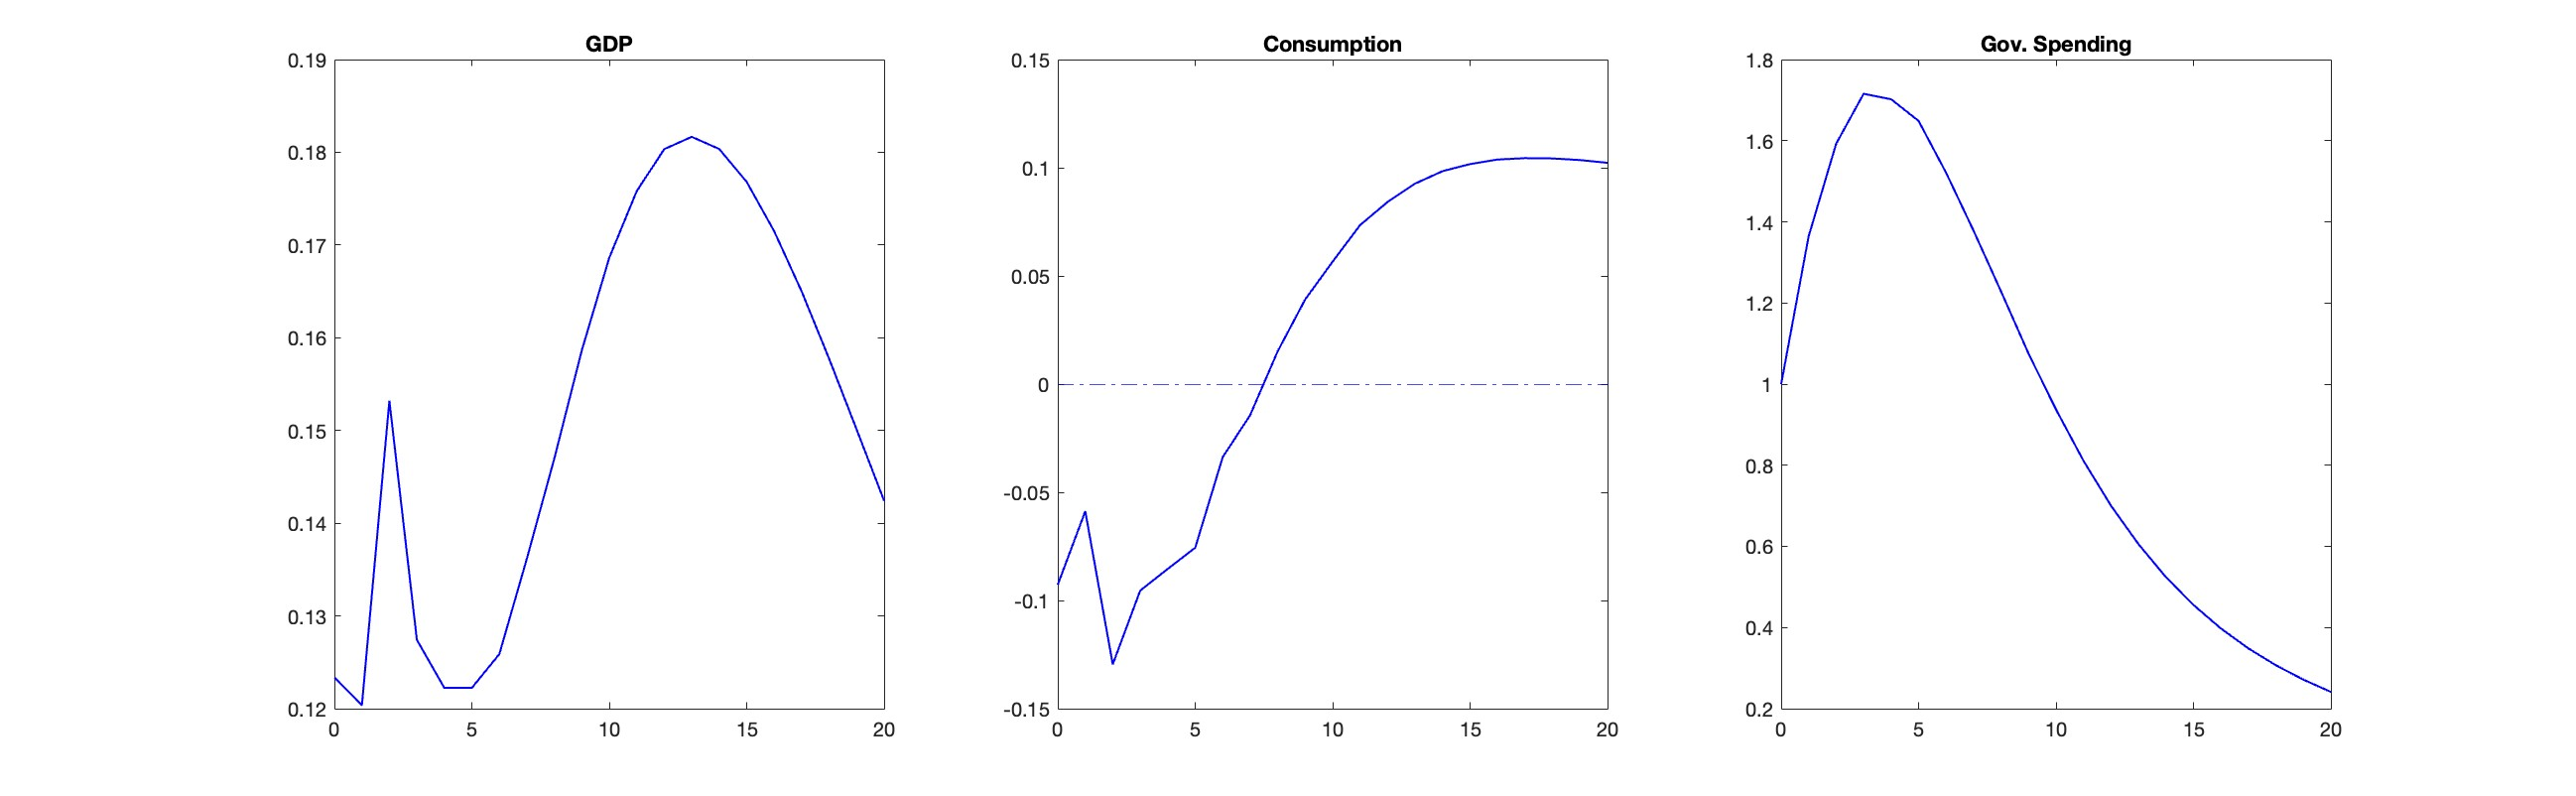
\includegraphics[width=1\linewidth]{Qb_1.jpg}
    \caption{Impulse Response Function for Government Spending Shock}
    \label{fig:enter-label}
\end{figure}

\end{CJK}
\end{document}